\documentclass[UTF8]{ctexart}
\usepackage{xcolor}
\usepackage{enumerate}
\usepackage{graphicx}
\usepackage{geometry}
\usepackage{graphicx} %插入图片的宏包
\usepackage{float} %设置图片浮动位置的宏包
\usepackage{subfigure} 
\usepackage[colorlinks,linkcolor=blue]{hyperref}
\usepackage{mathtools}
\usepackage{listings}
\lstset{ %
    language=python,                % the language of the code
    basicstyle=\footnotesize,           % the size of the fonts that are used for the code
    numbers=left,                   % where to put the line-numbers
    numberstyle=\tiny\color{gray},  % the style that is used for the line-numbers
    stepnumber=2,                   % the step between two line-numbers. If it's 1, each line 
                                    % will be numbered
    numbersep=5pt,                  % how far the line-numbers are from the code
    backgroundcolor=\color{white},      % choose the background color. You must add \usepackage{color}
    showspaces=false,               % show spaces adding particular underscores
    showstringspaces=false,         % underline spaces within strings
    showtabs=false,                 % show tabs within strings adding particular underscores
    frame=single,                   % adds a frame around the code
    rulecolor=\color{black},        % if not set, the frame-color may be changed on line-breaks within not-black text (e.g. commens (green here))
    tabsize=2,                      % sets default tabsize to 2 spaces
    captionpos=b,                   % sets the caption-position to bottom
    breaklines=true,                % sets automatic line breaking
    breakatwhitespace=false,        % sets if automatic breaks should only happen at whitespace
    title=\lstname,                 % show the filename of files included with \lstinputlisting;
                                    % also try caption instead of title
    keywordstyle=\color{blue},          % keyword style
    commentstyle=\color{green},       % comment style
    stringstyle=\color{red},         % string literal style
    escapeinside={\%*}{*)},            % if you want to add LaTeX within your code
    morekeywords={*,...}               % if you want to add more keywords to the set
}
\geometry{left = 2.5cm,right= 2cm}
\title{Chapter 2 \\End to End Machine Learning}
\author{DuLi}
\date{\today}
\begin{document}
\maketitle
\newpage
\tableofcontents
\newpage
\section{Outline}
\setlength{\parskip}{0.5em} 

Here are main steps you will go through:
\begin{itemize}
	\item[1.] Look at the big picture.
	\item[2.] Get the data.
	\item[3.] Discover and visualize the data to gain insights.
	\item[4.] Prepare the data fpr machine learning algorithms.
	\item[5.] Select a model and train it.
	\item[6.] Fine-tune your model.
	\item[7.] Present your solution.
	\item[8.] Launch,monitor,and maintain your system.
\end{itemize}
\section{Working with Real Data}
Here are a afew places you can look to get data:
\begin{itemize}
	\item Popular open data open repositories:
		\item[-] UC Irvine Machine Learning Repositories.
		\item[-] Kaggle datasets.
		\item[-] Amazon's AWS datasets.
	\item Meta Portals(they list open data repositories)
		\item[-] dataportals.org
		\item[-] opendatamonitor.eu
		\item[-] quandl.com
	\item Other pages listing many popular open data repositories
		\item[-] Wikipedia's list of Machine Learning datasets.
		\item[-] Quora.com question.
		\item[-] Datasets subreddit.
\end{itemize}

\begin{figure}[H]
\centering
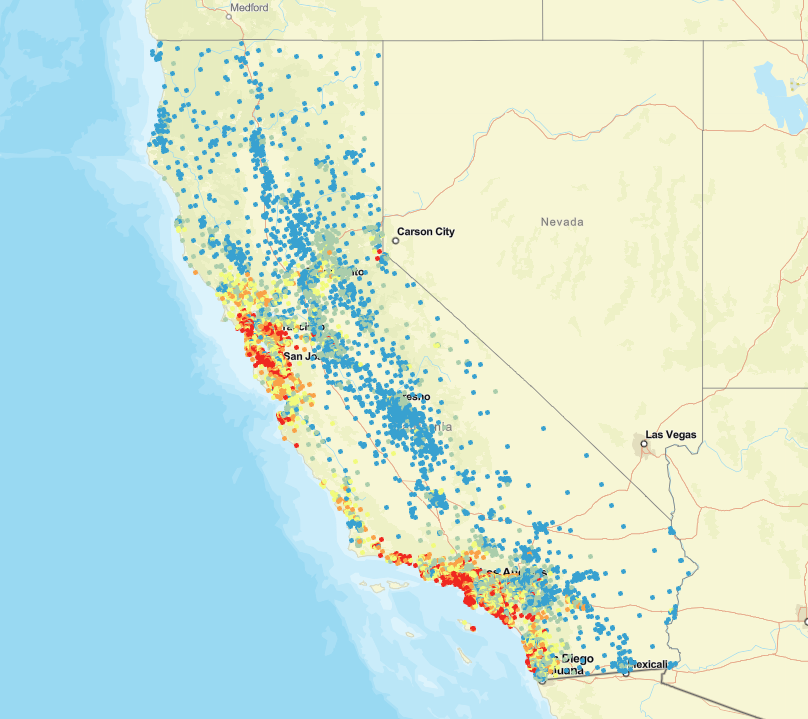
\includegraphics[width = 4in]{picture.png}
\caption{California Housing Prices Databases}
\end{figure}

\section{Look at the Big Picture}
\subsection{Frame the Problem}
The first question to ask you is what exactly is the bussiness objective;building a model is probably not the end goal.How do you expect use and benefit from this model?This is improtant because it will determine how you frame the problem,what algorithms you will select,what performance measure you will use to evaluate your model,and how much effort you should spend tweaking it.
Your model output (a predicting of a district's median housing price) will be fed to another Machine Learning system along with many other signals.This downstream system will determine whether it is worth investing in a given area or not.

\begin{figure}[H]
\centering
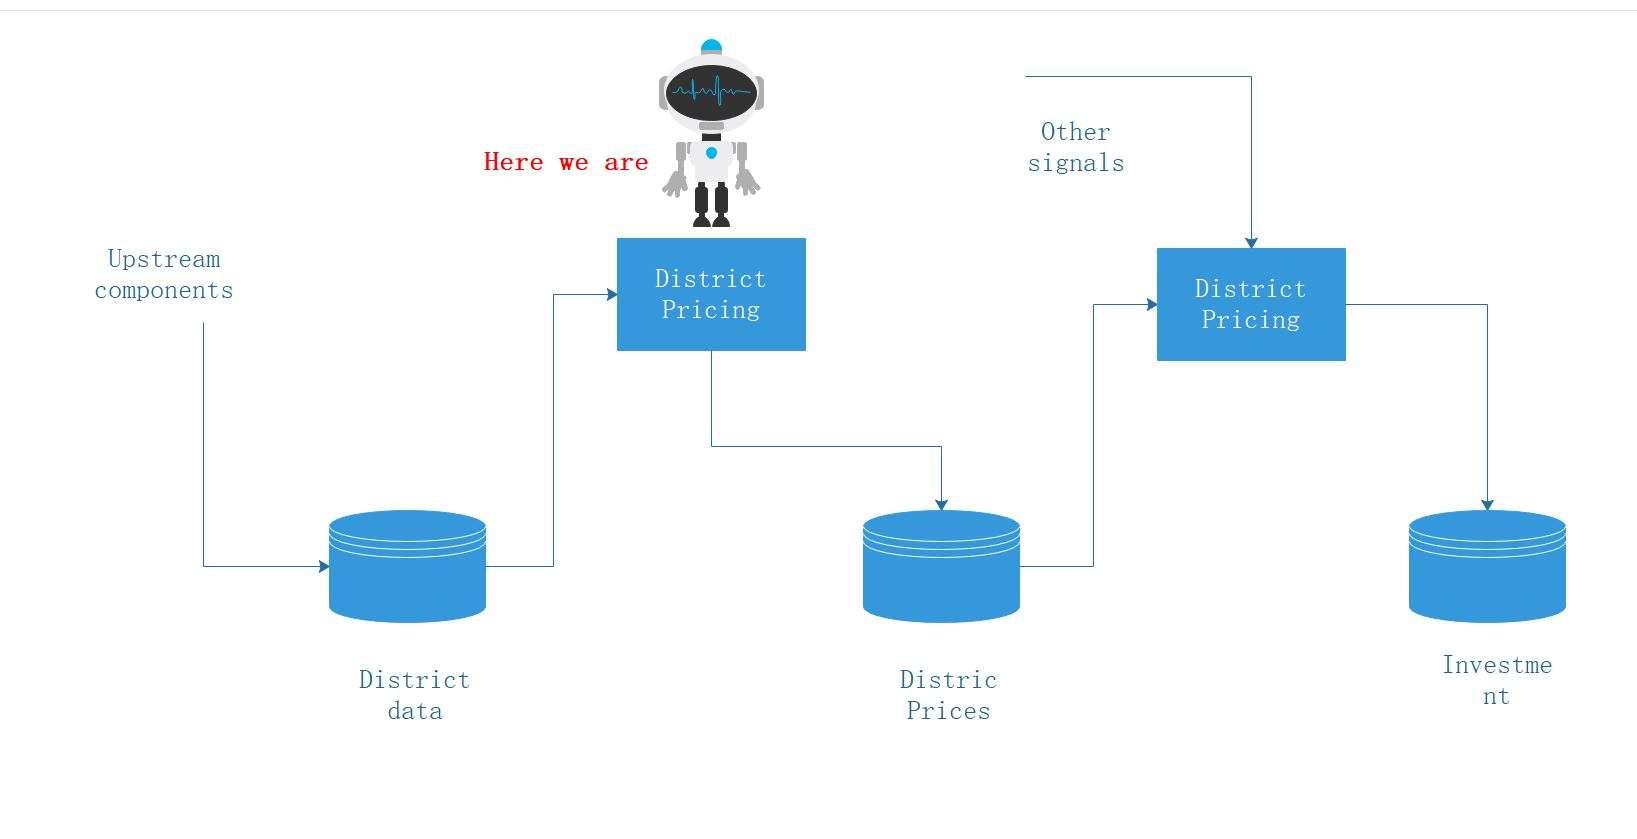
\includegraphics[width = 4in]{PROCESS.JPG}
\caption{A machine learning pipeline for real estate investment}
\end{figure}

The next step is framing the problem:is it supervised,unsupervised,or Reinforcement learning?Is it a classification task,a regression task,or something else?Should we use batch learning or online learning technique?
Clearly it is supervised,we need historical data to train the model.Moreover it is a typical regression task,more specifically,this is a multivariate regression since the system will use mutiple features to make a prediction.In first chapter,we predicted life satisfiction based on just one feature,the GDP per captia.Finally,there is no continuous flow of data coming in the system,there is no particular need to adjust to changing data rapidly,and the data is small enough to fit in memory,so plain batch learning should do just fine.

\subsection{Select a Performance Measure}
The next step is to select a performance measure.A typical performance measure for regression problems is the Root Mean Square Error(均方根误差),it measures the standard deviation of the errors the system makes in its prediction.

\begin{equation}
RMSE(X,h) = \sqrt{\frac{1}{m}\sum_{i=1}^{m}(h(X^{i})-y^{i})^{2}}
\end{equation}

Even though the RMSE is generally the perferred performance measure for regression tasks,in some contexts you may prefer to use another function.For example,suppose that there are many outlier districts.In that case,we may consider using the Mean Absolute Error(平均绝对误差):
\begin{equation}
	MAE(X,h) = \frac{1}{m}\sum_{i=1}^{m}|h(X^i)-y^i|
\end{equation}

Both the RMSE and MAE are ways to measure the \emph{distance} between two vectors.Various distance measures or norms are possible:
\begin{itemize}
	\item Euclidean norm(欧几里得距离)。
	\item Manhattan norm(曼哈顿距离),it measures the distance between two points in a city if you can only travel along orthogonal city blocks.也就是指城市中两点之间沿着街区边缘走路的距离。
	\item More generally,the $l_{k}$ norm of a vector $v$ containing n elements is defined as:
	\begin{equation}
		\parallel v \parallel = (\mid v_{o} \mid^k + \mid v_{1} \mid^k+ \cdots + \mid v_{n} \mid^k)^\frac{1}{k} 
	\end{equation}
\end{itemize}

\section{Get the data}
It's time to get your hands dirty.
\subsection{Create the workspace}
First,you need to have Python enviornment installed.We recommand you installed anaconda on your computer.\url{https://www.anaconda.com/}
\subsection{Take a Quick Look at the Data Structure}
Let's take a look a the Data Structure.I download the database from Kaggle.\url{https://www.kaggle.com/camnugent/california-housing-prices}.Let's take a glance of the data structure.
Each row represent one district.There are 10 attributes(Figure 3):longitude,lattidute,housing\underline{ }median\underline{ }age,total\underline{ }\\rooms,total\underline{ }bedrooms,population,households,median\underline{ }income,median\underline{ }house\underline{ }value,ocean\underline{ }proximity.

\begin{figure}[H]
\centering
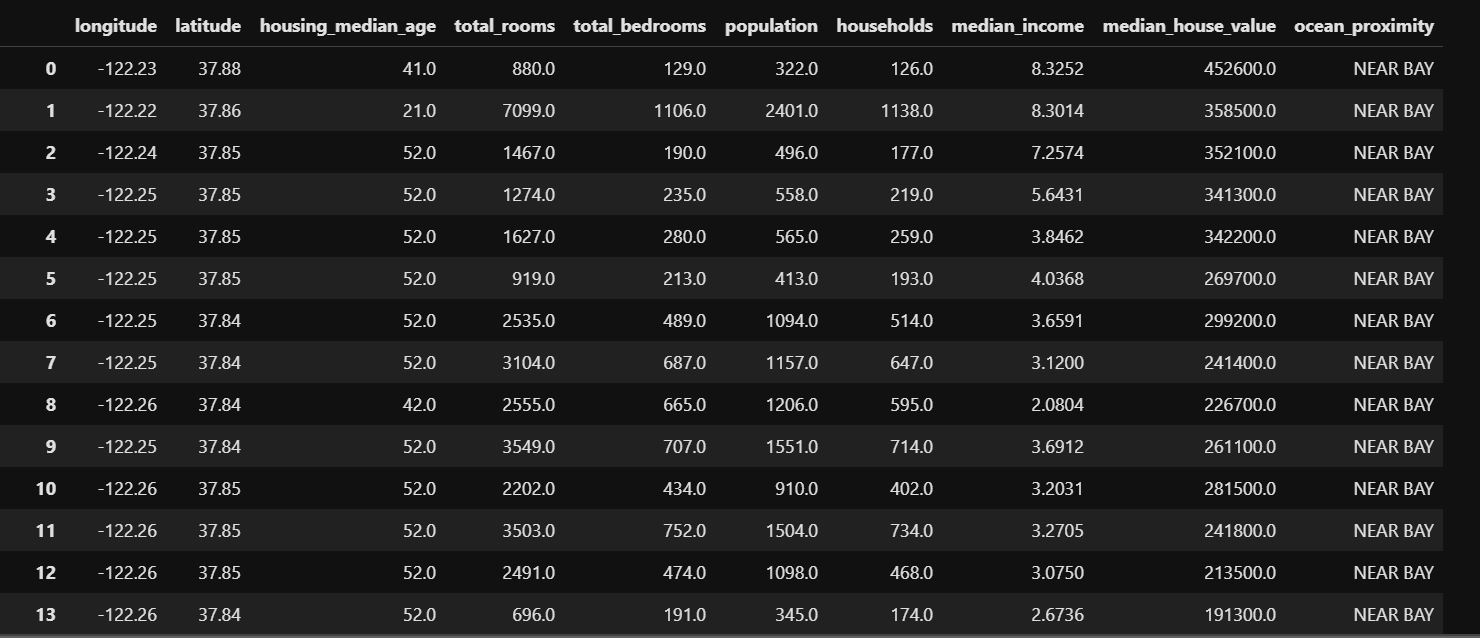
\includegraphics[width = 4in]{DataStructure.JPG}
\caption{Data Structure}
\end{figure}

The info method is useful to get a quick description of the data,in particular the total number of rows,and each attribute's type and number of non-null values.There are 20640 instances in the dataset,which means that it is fairly small by Machine Learning standards,but it's perfect to get started.Notice that the total\underline{ }bedrooms attribute has only 20433 non-null values,meaning that 207 districts are missing this feature.We will need to take care of this later.

\begin{figure}[H]
\centering
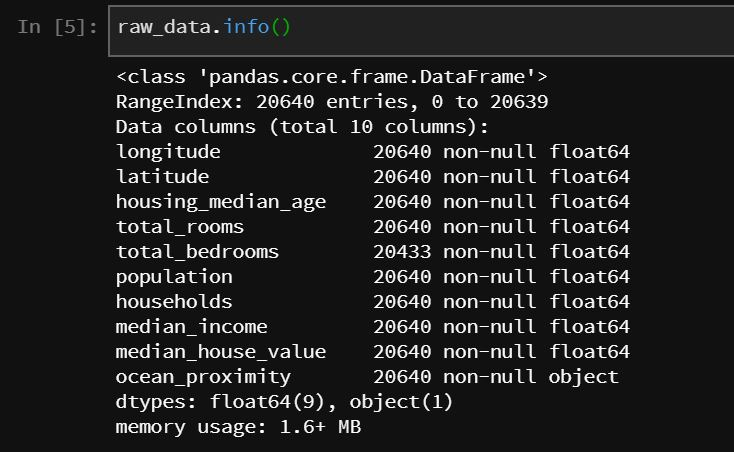
\includegraphics[width = 4in]{datainfo.JPG}
\caption{Data Info}
\end{figure}

All attribute are numercial,except the ocean\underline{ }proximity field.We can find out what categories exist and how many districts belong to each category by using the value\underline{ }counts() method:

\begin{figure}[H]
\centering
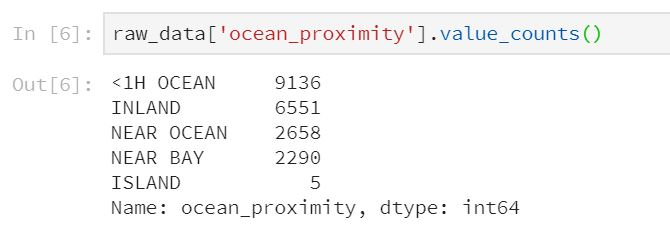
\includegraphics[width = 3in]{datacounts.JPG}
\caption{Data Counts}
\end{figure}

Let's look at the other fields.The describe() method shows a summary of the numercial attributes.(Figure 6).The count,mean,min and max rows are self-explanatory.

\begin{figure}[H]
\centering
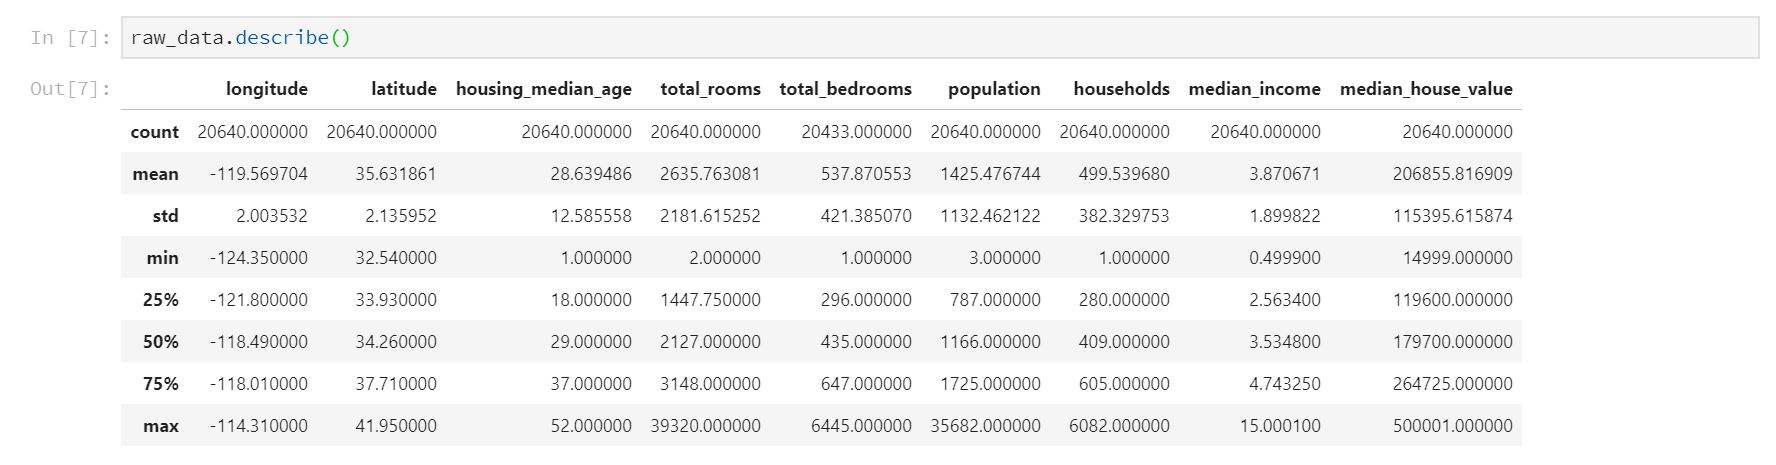
\includegraphics[width = 4in]{DATADESCRIBE.JPG}
\caption{Data Describe}
\end{figure}

Another quick way to get a feel of the type of data you are dealing with is to plot a histogram for each numercial attribute.

\begin{figure}[H]
\centering
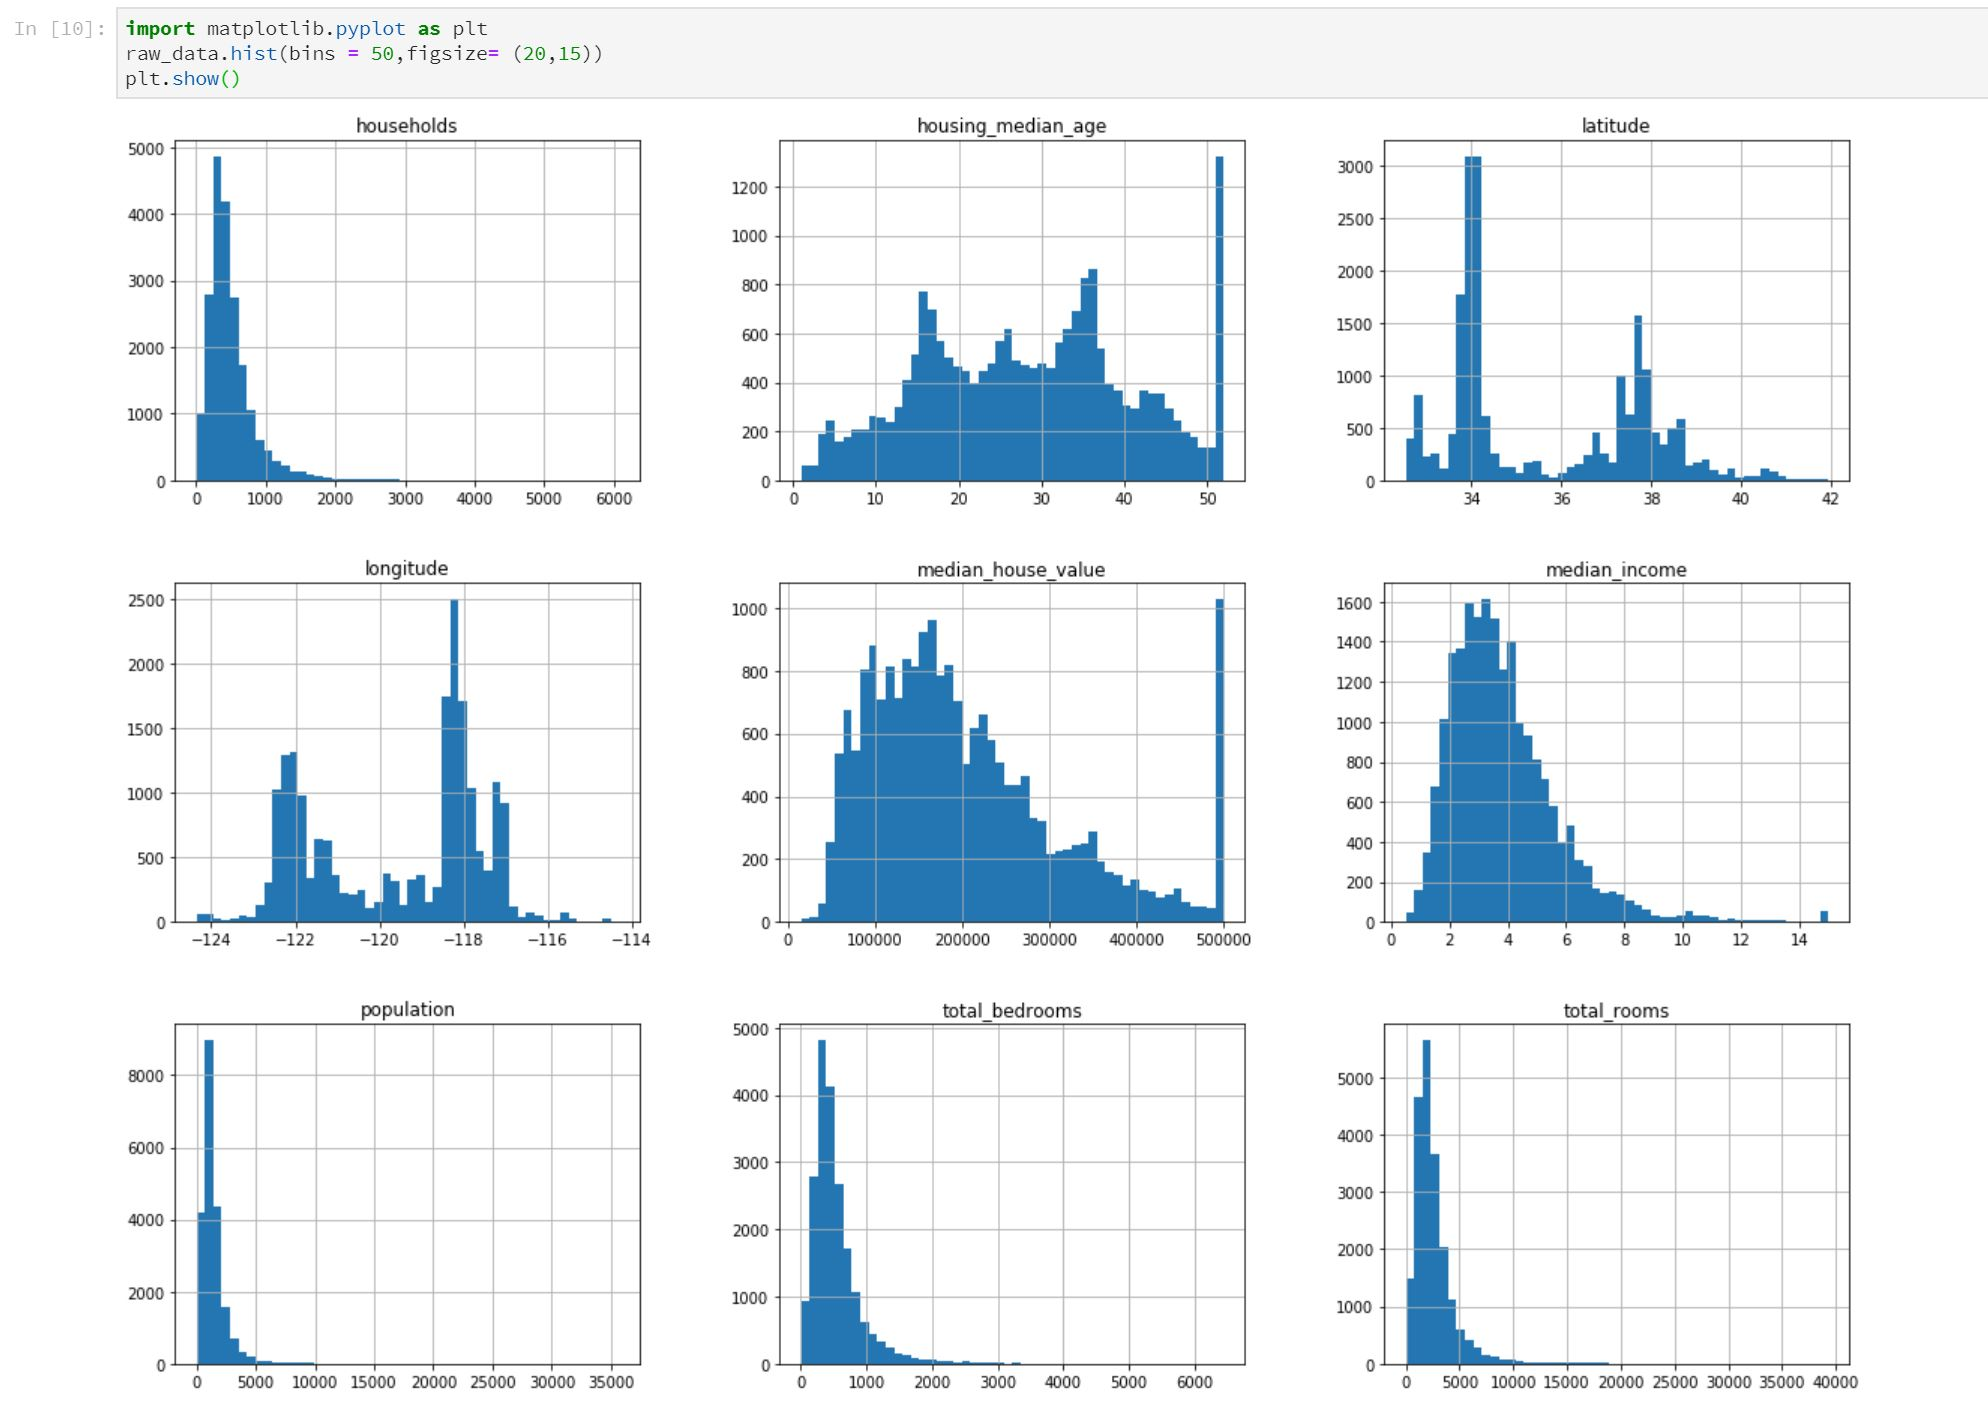
\includegraphics[width = 3.5in]{datahist.JPG}
\caption{A histogram for each numercial attribute}
\end{figure}

\subsection{Create a Testset}

Create a test set is theoretically quite simple:just pick some instances randomly,typically 20\% of the dataset,and set them aside.

\begin{lstlisting}
import numpy as np

def split_train_test(data,test_ratio):
	shuffled_indices = np.random.permutation(len(data))
	test_set_size = int(len(data)*test_ratio)
	test_indices = shuffled_indices[:test_size]
	train_indices = shuffled_indices[test_size:]
	return data.iloc[train_indices],data.iloc[test_indices]

\end{lstlisting}

We can then using the function like this:
\begin{lstlisting}
train_set,test_set = split_train_test(housing,0.2)
\end{lstlisting}

This works,but it not perfect:if you run the program again,it will generate a different test set.One solution is to save the test set on the first run and then load it in subsequent runs.Another option is to set the random number generate's seed(eg. np.random.seed(52))before calling np.permutation().But both these solution will break next time you fetch an updated dataset.A common solution is to use each instance's identifier to decide whether or not it should go in the test set.For example,you could compute a hash of each instance's identifier.

\begin{lstlisting}
import hashlib

def test_set_check(identifier,test_ratio,hash):
    return hash(np.int64(identifier).digest()[-1]<256*test_ratio)

def split_train_test_by_id(data,test_ratio,id_column,hash=hashlib.md5):
    ids = data[id_column]
    in_test_set = ids.apply(lambda id_:test_set_check(id_,test_ratio,hash))
    return data.iloc[~in_test_set],data.iloc[in_test_set]
\end{lstlisting}

Unfortunately,the hosuing dataset does not have an identifier column.The simplest solution is to use the row index as the ID:
\begin{lstlisting}

housing_with_id = housing.reset_index()
train_set,test_set = split_train_test_by_id(hosuing_with_id,0.2,"index")

\end{lstlisting}


We can utilize the train\underline{ }test\underline{}split function to reah the same effect of the split function above.

\begin{lstlisting}
from sklearn.model_selection import train_test_split

train_set,test_set = train_test_split(housing,test_size = 0.25,random_state = 0)

\end{lstlisting}
This generally fine if your dataset is large enough,bu if it is not,you run the risk of introducing a significant sampling bias.For example,when a survey company decides to call 1000 people to ask them a few questions ,they don't just pick 1000 people randomly in a phone booth.They try to ensure that these 1000 people are representative of the whole population,eg. the US population is composed of 51.3\% female and 48.7\% male,so a survey in the US should try to maintain this ratio in the sample:513 female and 487 male.This is called \emph{stratified sampling.}

Since the median income is a very important attribute to predict median housing prices. You may want to ensure that the test set is representative of the various categories of incomes in the whole dataset 

\begin{figure}[H]
\centering
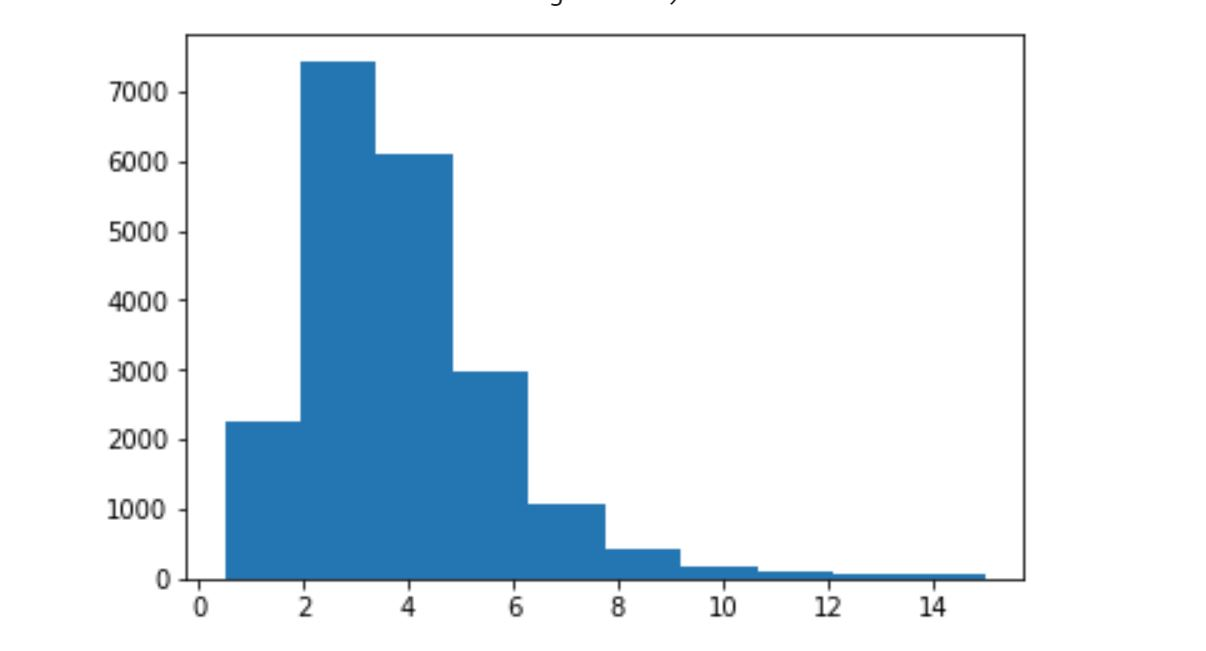
\includegraphics[width = 4in]{incomehist.JPG}
\caption{Histogram of income categories}
\end{figure}

Let's look at the histogram of income categories,most median income values are clustered around 2-5(tens of thousands of dallors),but some median incomes go far beyond 6.It is important to have a sufficient number of instances in your dataset for each stratum,or else the estimate of the stratum'simportance may br biased,so we should not have too many strata(dividing the median income by 1.5 and rounding up using cel and then merge all the categories greater than 5 into category 5).

\begin{lstlisting}
raw_data["income_cat"] = np.ceil(raw_data["median_income"]/1.5)
raw_data["income_cat"].where(raw_data["income_cat"]>5,5.0,inplace = False)
\end{lstlisting}

Now you are ready to do stratified sampling based on the income category.For this we can use Scikit-learn's StratifiedShuffleSplit class:

\begin{lstlisting}
from sklearn.model_selection import StratifiedShuffleSplit

split = StratifiedShuffleSplit(n_splits = 1,test_size = 0.2, random_state = 17)

for train_index, test_index in split.split(raw_data, raw_data["income_cat"]):
    strat_train_set = raw_data.loc[train_index]
    strat_test_set = raw_data.loc[test_index]	
\end{lstlisting}

By this way,the category proportions in the test\underline{ }set which generated with stratified sampling almost identical to those in the full dataset.

We spent quite a bit of time on the test set generation for a good reason:this is an often neglected but critical part of a Machine Learning project.
At last,we should remove the income\underline{ }cat attribute so the data is back to its original state:

\begin{lstlisting}
for set in(strat_train_set,strat_test_set):
	set.drop(["income_cat"],axis = 1,inplace = True)
\end{lstlisting}


这个部分看似平淡无奇,其实还蛮有用的,之前在选数据集的时候,从来没有考虑过这个问题。回头想想,选择有代表性的数据集对于一个监督学习的系统来说,还是非常重要的。使得在训练阶段也能提高精度,这个道理我想是不言自明的。

\section{Discover and Visualize the Data ti Gain Insights}

So far we have only taken a quick glance at the data to get a general understanding of the kind of data we are manipulating.In our case,the set is quite small so you can just work directly on the full set.Let's create a copy so you can play with it without harming the training set.

\begin{lstlisting}
housing = strat_train_set.copy()
\end{lstlisting}

\subsection{Visualizing Geographical Data}

Since there is geographical information(latitude and longitude),let's plot it!

\begin{lstlisting}
housing.plot(kind="scatter",x="longitude",y="latitude")
\end{lstlisting}

\begin{figure}[H]
\centering
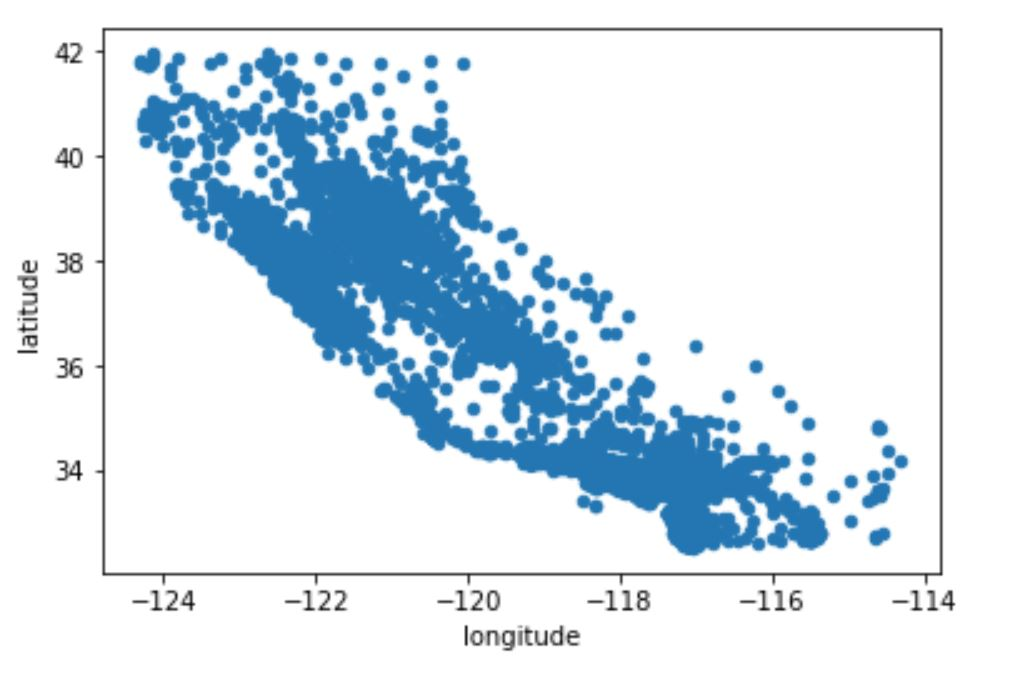
\includegraphics[width = 4in]{longi_and_lati.JPG}
\caption{A geographical scatterplot of the data}
\end{figure}

Setting the alpha option to 0.1 makes it much easier to visualize the places where there is a high density of data points.

\begin{lstlisting}
housing.plot(kind="scatter",x="longitude",y="latitude",alpha = 0.1)
\end{lstlisting}

alpha:float (0.0 transparent through 1.0 opaque),这里的alpha指的是透明度,所以密度越大的地方,因为重叠的原因,颜色就会越深。

It's better now,let's look at the housing prices.The radius of each circle represents the district's population(option s),and the color represents the price(option c).We will use a predefined color map(option cmap)called jet,which ranges from blue(low values) to red(high prices):

\begin{lstlisting}
housing.plot(kind="scatter",x="longitude",y="latitude",alpha=0.4,s=housing["population"]/100,label="population",c="median_house_value",cmap=plt.get_cmap("jet"),colorbar=True)
plt.legend()
\end{lstlisting}

\begin{figure}[H]
\centering
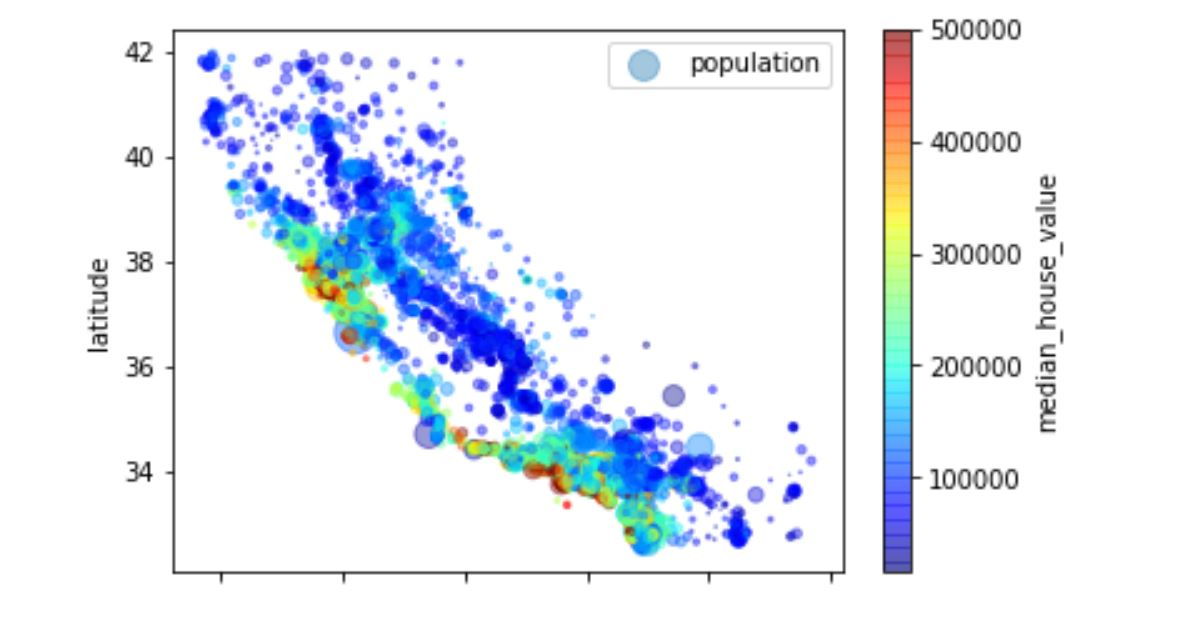
\includegraphics[width = 4in]{Housing_price_pic.JPG}
\caption{California housing prices}
\end{figure}

观察最后得到的图我们大概能看得出一些结论,这些结论也与我们的常识相符。首先,房价和位置的关系很大,临海的房价普遍要高一些,还有某些位置的房价普遍要高一些,这些地方应该是加州沿海的一些城市,旧金山,洛杉矶等等。当然这也不是全部,北部沿海的房价也会低一些。

\subsection{Looking for Correlations}

 Since the data set is not too large ,we can easily compute the \emph{Standard correlation coefficient}(also called Pearson's r 皮尔森相关系数) between every pair of attributes using the corr() method:

\begin{lstlisting}
corr_matrix = housing.corr()
\end{lstlisting}

The matrix is big,so let's look at a specific attribute(eg.median house value).
\begin{lstlisting}
corr_matrix["median_house_value"].sort_values(ascending=False)
\end{lstlisting}

The correlation coefficient ranges from 1 to -1.接近1代表正相关,接近-1代表负相关,我们可以看出平均房价和收入是正相关关系,而和经度是负相关的,也就是内陆房价低,沿海高。Finally,coefficients close to zero mean there is no linear correlation.

\begin{figure}[H]
\centering
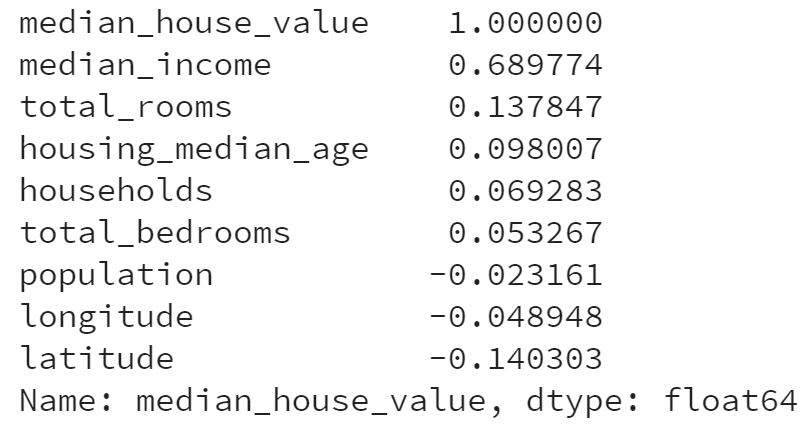
\includegraphics[width = 2.5in]{pearson_r.JPG}
%\caption{California housing prices}
\end{figure}

下面这张图来自维基百科,从左到右依次表示皮尔森相关系数在不同值时的情况。

\begin{figure}[H]
\centering
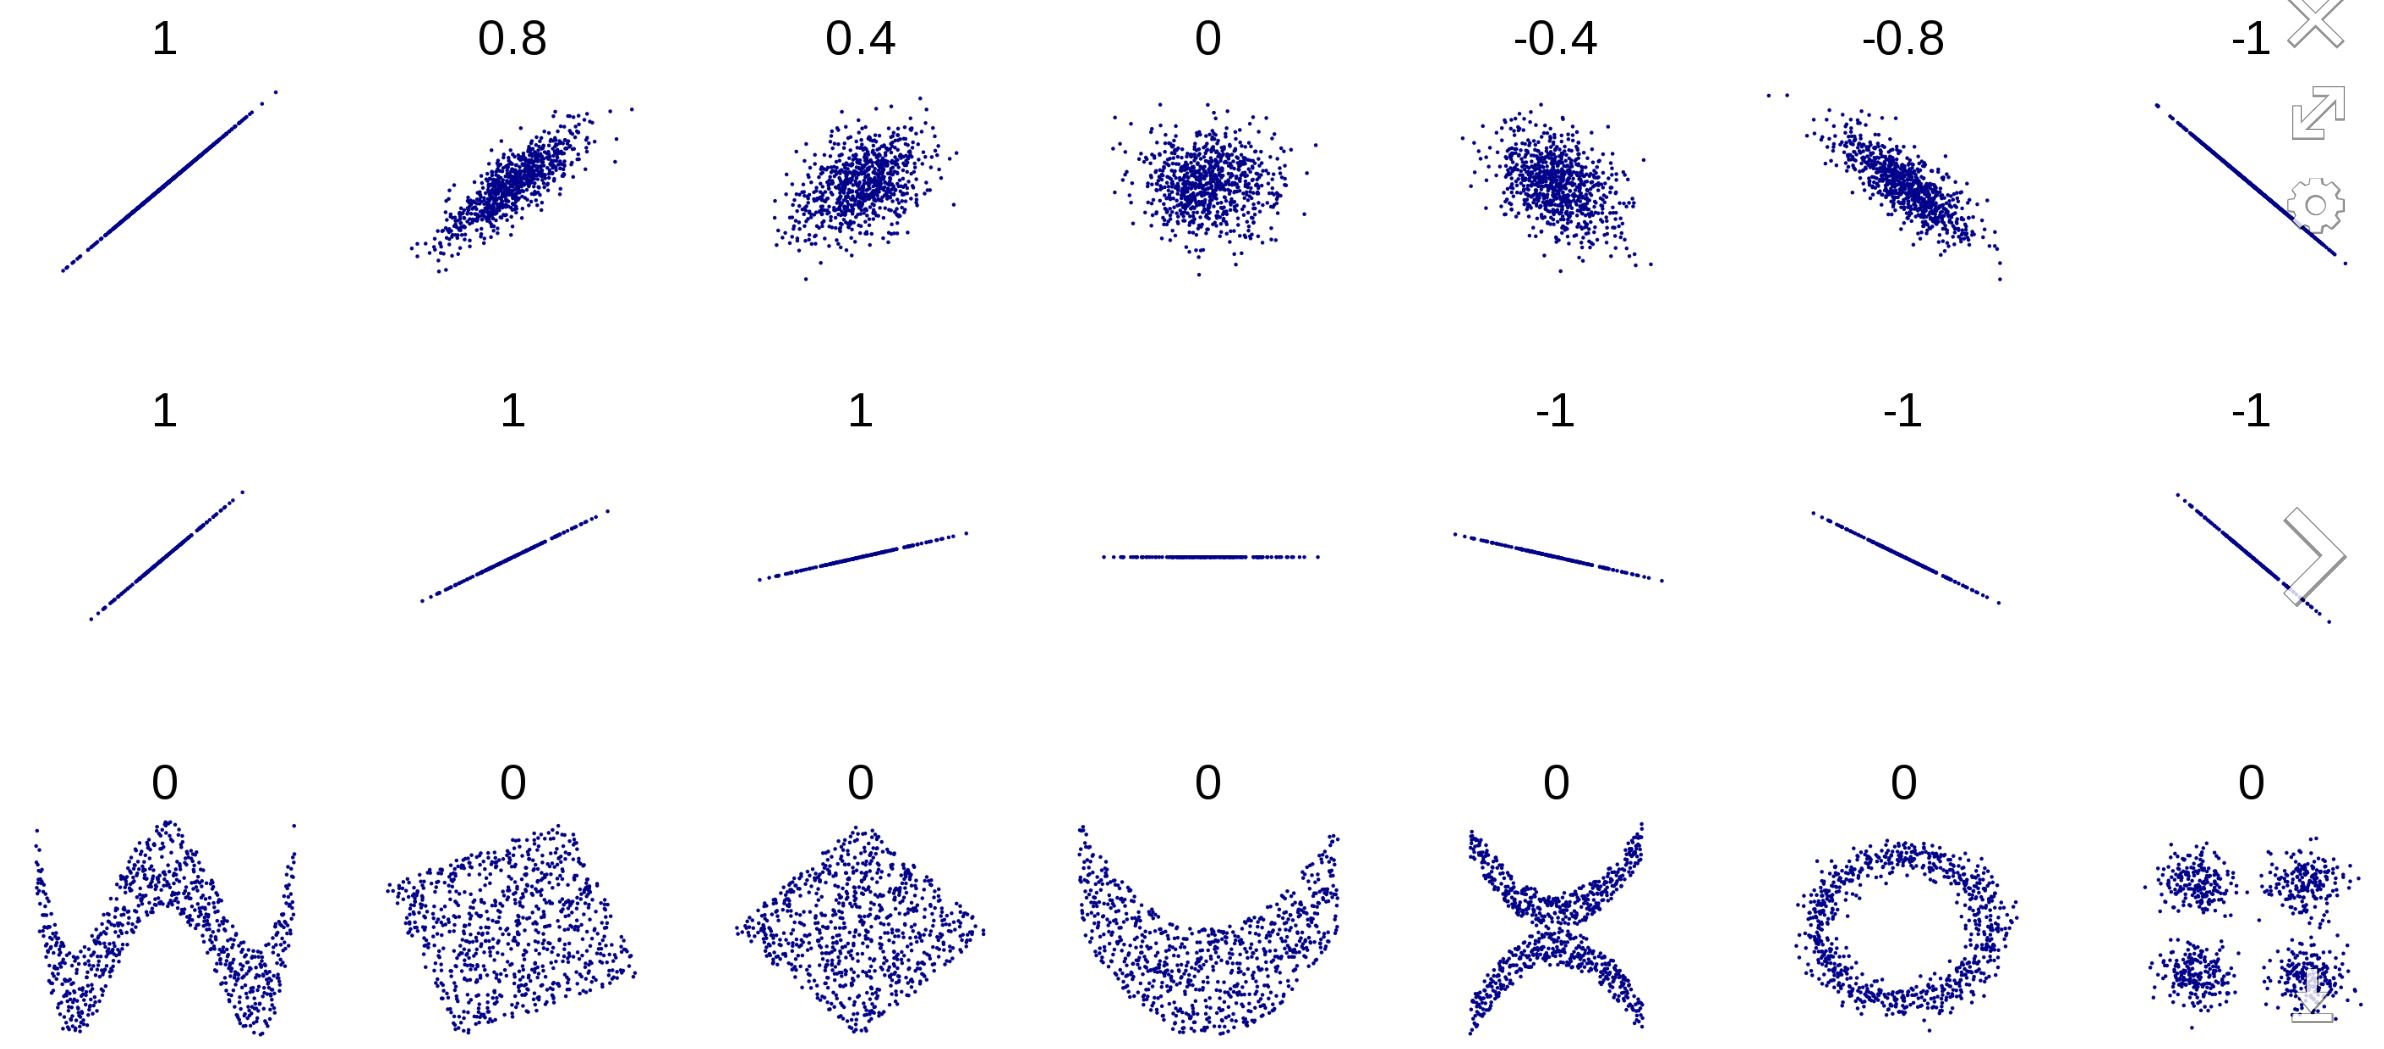
\includegraphics[width = 4in]{scatter_matrix.JPG}
\caption{Scatter Matrix}
\end{figure}

The correlation coefficient only measures linear correlations.

Another way to check for correlations between attributes is to use Pandas' scatter\underline{ }matrix function.Since there are now 11 numerical attributes,you would get $11^2$ plots,so let's just focus on a few promising attributes that seem most correlated with the median housing value.

\begin{lstlisting}
from pandas.plotting import scatter_matrix

attributes = ["median_house_value","median_income","total_rooms","housing_median_age"]

scatter_matrix(housing[attributes],figsize=(12,8))
\end{lstlisting}


\begin{figure}[H]
\centering
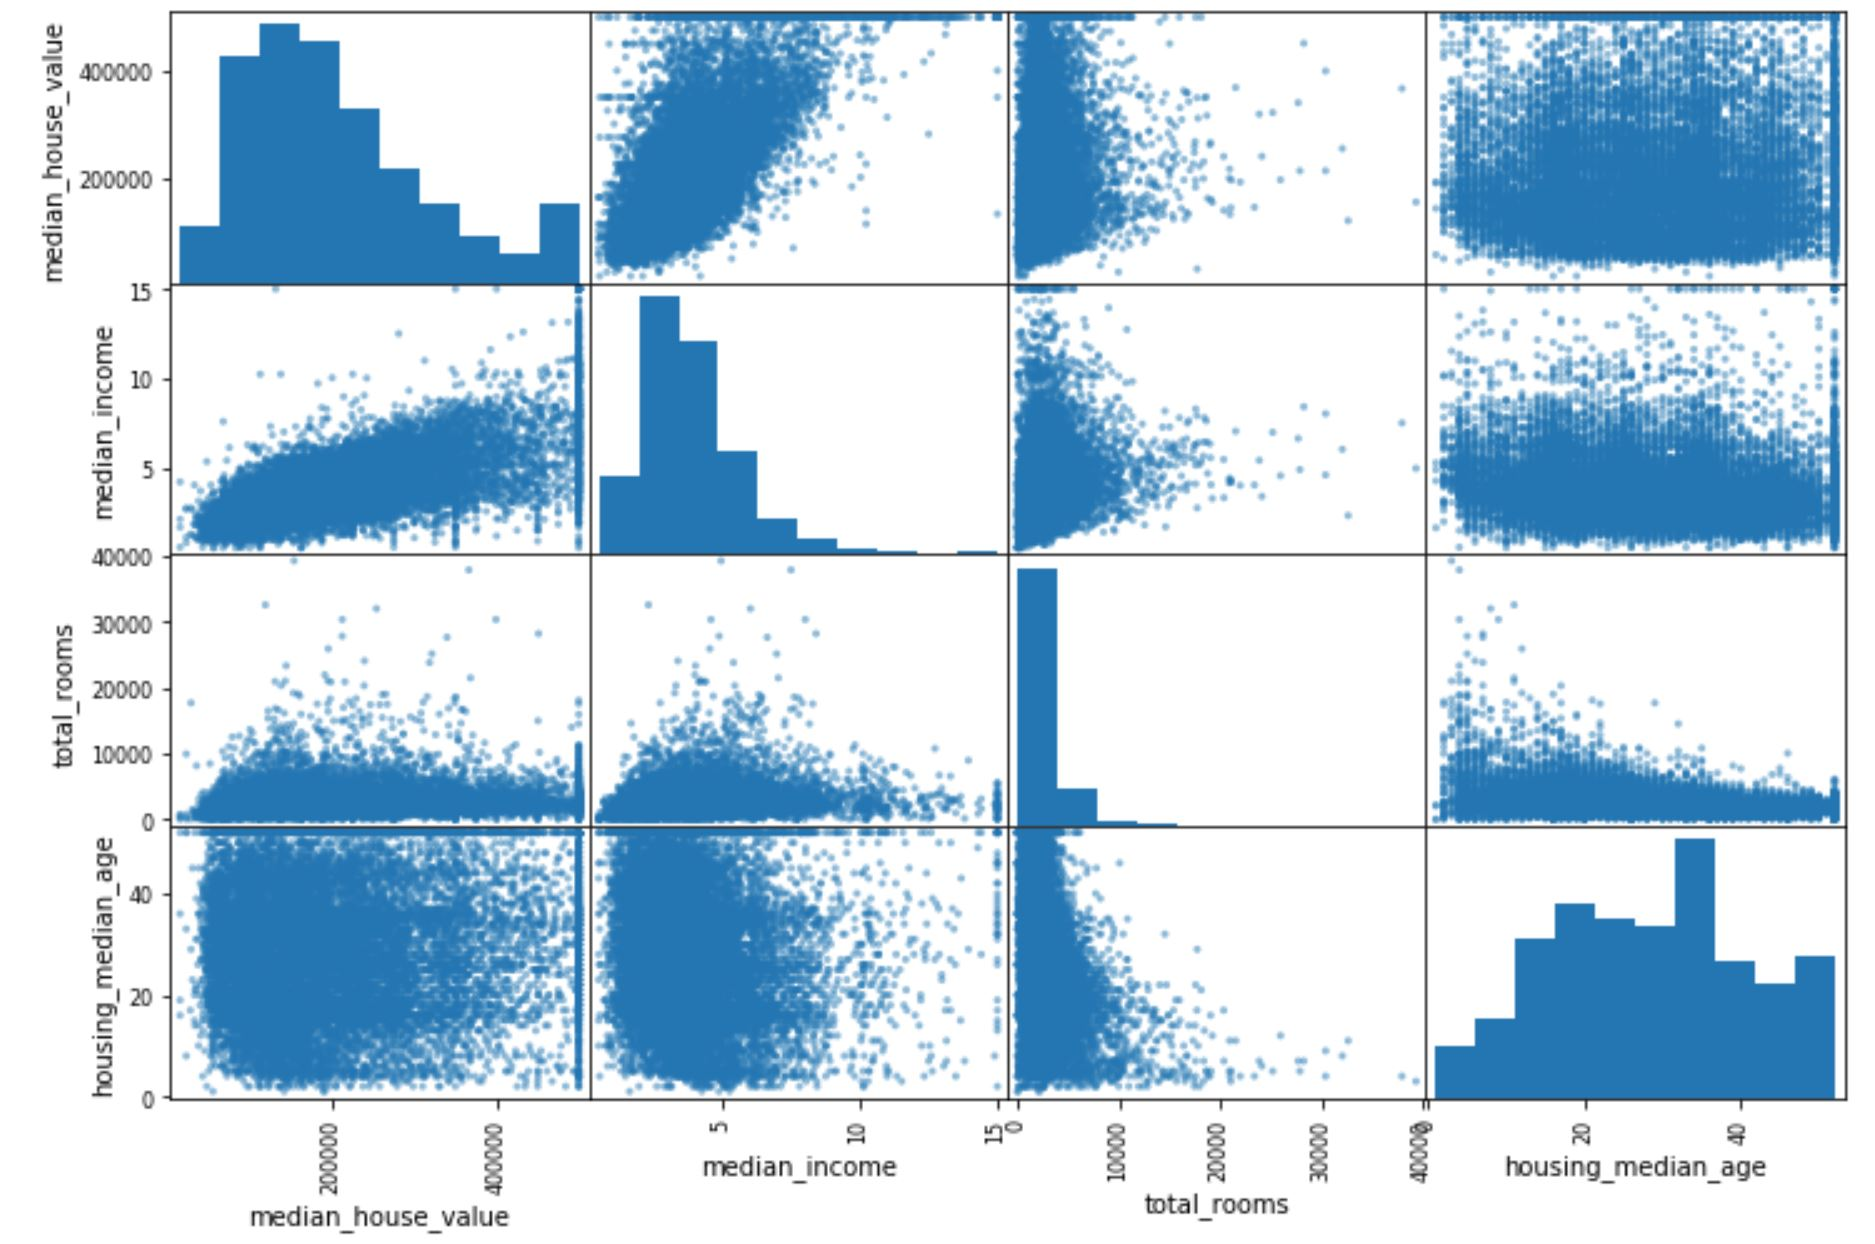
\includegraphics[width = 4in]{scatter_col.JPG}
\caption{Scatter Matrix}
\end{figure}



\end{document}
